\documentclass{article}
\usepackage{tikz}
\usetikzlibrary{patterns}
\usetikzlibrary{decorations.pathmorphing}

\begin{document}
    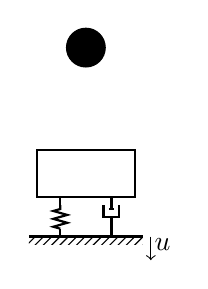
\begin{tikzpicture}
        \draw[black,thick] (-0.1,0) -- (1.35, 0);

        %Schraffur einfügen
        \fill[pattern = north east lines] (-0.1, -0.1) rectangle (1.35, 0);

        \draw[black, thick] (0, 0.5) rectangle (1.25, 1.1);

        %zigzag Linie, unten 
        \draw[black, thick] (0.3, 0.4) -- (0.3, 0.5);
        \draw[black, thick] (0.3, 0) -- (0.3, 0.1);
        \draw[black, thick, decorate, decoration = {zigzag, segment length = 1mm}] (0.3, 0.1) -- (0.3, 0.4);

        %neben zigzag, unten
        \draw[black, thick] (0.95, 0) -- (0.95, 0.25);
        \draw[black,thick] (0.95, 0.5) -- (0.95, 0.35);
        \draw[black,thick] (0.98, 0.35) -- (0.92, 0.35);
        \draw[black, thick] (0.85, 0.4) -- (0.85, 0.25) -- (1.05, 0.25) -- (1.05, 0.4);

        \draw[->] (1.45, 0) -- (1.45, -0.3);
        \draw (1.6, -0.1) node {$u$};

        %zigzag Linie, oben
        %\draw[black, thick] (0.625, 1.1) -- (0.625, 1.2);
        %\draw[black, thick] (0.625, 1.7) -- (0.625, 2);
        %\draw[black, thick, decorate, decoration = {zigzag, segment length = 1mm, amplitude = 2mm}] (0.625, 1.2) -- (0.625, 1.7);

        \filldraw[black] (0.625, 2.4) circle (7pt);

    \end{tikzpicture}
\end{document}